\documentclass{article}
\usepackage[final]{nips_2016} % produce camera-ready copy
% if you need to pass options to natbib, use, e.g.:
\PassOptionsToPackage{numbers, compress}{natbib}
% before loading nips_2016
%
% % to avoid loading the natbib package, add option nonatbib:
% \usepackage[nonatbib]{nips_2016}

% \usepackage{nips_2016}

% % to compile a camera-ready version, add the [final] option, e.g.:
% \usepackage[final]{nips_2016}

\usepackage[utf8]{inputenc} % allow utf-8 input
\usepackage[T1]{fontenc}    % use 8-bit T1 fonts
\usepackage{hyperref}       % hyperlinks
\usepackage{url}            % simple URL typesetting
\usepackage{booktabs}       % professional-quality tables
\usepackage{amsfonts}       % blackboard math symbols
\usepackage{nicefrac}       % compact symbols for 1/2, etc.
\usepackage{microtype}      % microtypography
\usepackage{amsmath}
\usepackage{mathtools}
\title{Deep Learning Assignment 4}

% The \author macro works with any number of authors. There are two
% commands used to separate the names and addresses of multiple
% authors: \And and \AND.
%
% Using \And between authors leaves it to LaTeX to determine where to
% break the lines. Using \AND forces a line break at that point. So,
% if LaTeX puts 3 of 4 authors names on the first line, and the last
% on the second line, try using \AND instead of \And before the third
% author name.
\author{
  Peter Yun-shao Sung
  \texttt{yss265@nyu.edu} \\
  %% examples of more authors
  %% \AND
  %% Coauthor \\
  %% Affiliation \\
  %% Address \\
  %% \texttt{email} \\
  %% \And
  %% Coauthor \\
  %% Affiliation \\
  %% Address \\
  %% \texttt{email} \\
  %% \And
  %% Coauthor \\
  %% Affiliation \\
  %% Address \\
  %% \texttt{email} \\
}

\begin{document}
% \nipsfinalcopy is no longer used

\maketitle
\section{Warmup}
\begin{figure}[h]
\centering
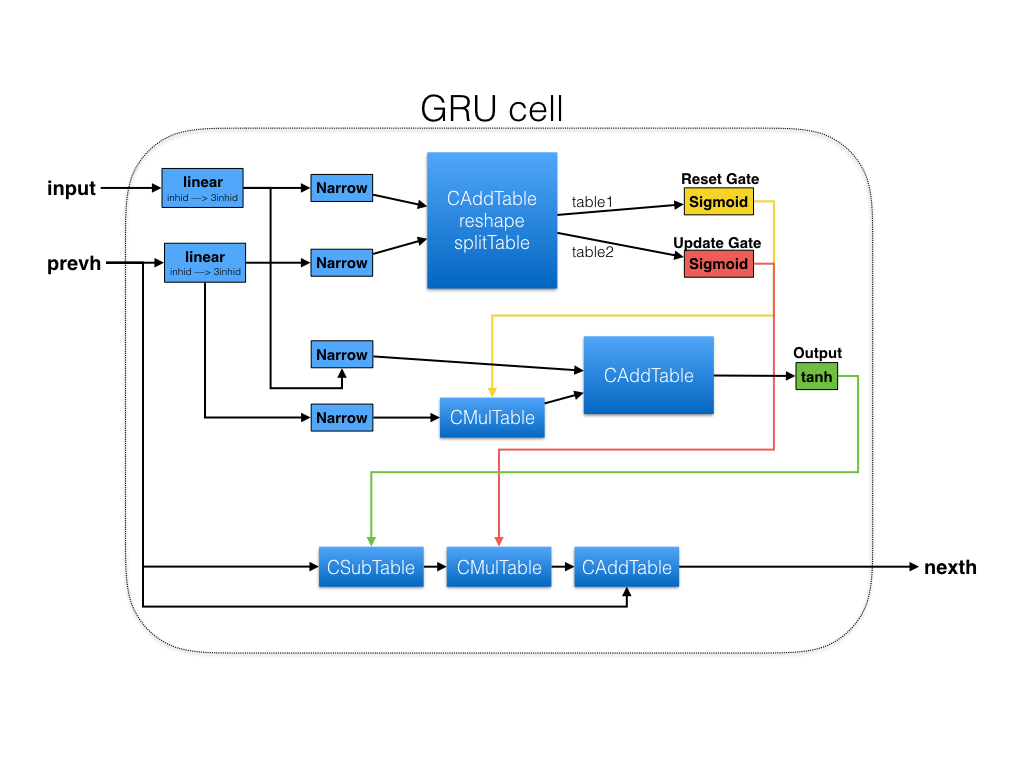
\includegraphics[width=70mm]{../q2/q2.png}
  \caption{GRU cell unit}
\end{figure}

\section{Approaches to RNN}
\subsection{Architecture}
The initial model is based on lstm as building block, with 2 layers and 20 sequence length. Layers are horizontally considering the current given input (or word) and the states passed from previous sequence. Sequence is the stack of multiple layers, and is used for vertically passing states to the next layers. This way, model can not only predict the next word based on current word (horizontal), but the predictions can be altered based on the sequence of previous words (vertical). Regarding to each lstm layer, there are number of rnn\_size lstm unit, and each of the unit perform the operation shown as figure 1.

\begin{figure}[h]
\centering
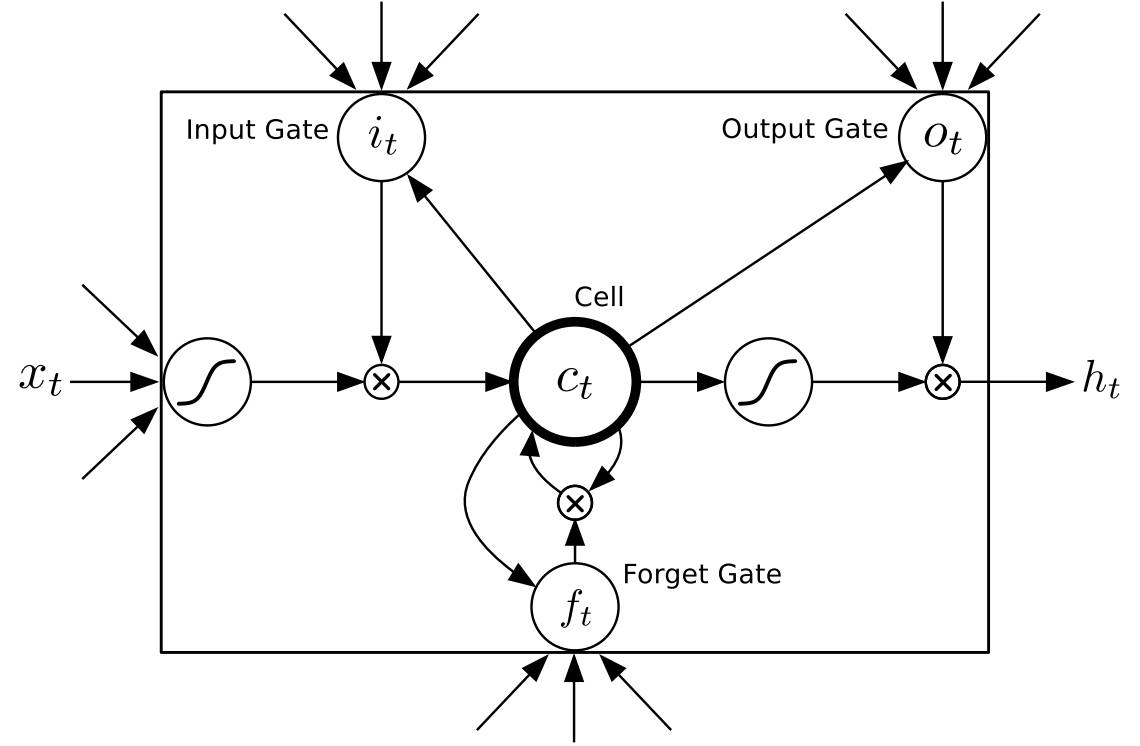
\includegraphics[width=30mm]{./fig/lstm.png}
  \caption{Operation of each of lstm unit}
\end{figure}

\subsection{Learning Techniques}
The two main learning techniques were the dropout and gradient clip. Dropout method was applied between each of lstm module and the final output. The inital module didnot used the dropout, and therefore we can observed that the perplexity of training improved well but not for the validation. This implies the concerns of overfitting and dropout might be a good option to improve.\\
Gradient clipping might be important method during the learning process too. Soft-clipping was initially applied to the model, which it observes the L2 norm of gradient and every gradient will multiply the portions it overpassed if the norm is higher than the threshold. The other method I used during this assignment is hard clipping, which we only cut the gradiend for only the one that pass threshold, instead of the every gradients. The inspiration is mainly from the curiousity of whether soft clipping downgrade the learning process for other gradient. However, as designing gridient checker and tracking perplexity, I noticed simply cut the gradient that overpassed might be problematic, as there might be also many gradients need to cut and it turns out every gradients are at the boarder line, and this make generally high gradient and high perplexity.

\subsection{Training Procedure}
Data was preprocessed in the shape of (lines,batch\_size), which is basically to traing a batch size of words. During each forward or backward propagation, line $i$ and $i+1$ is the corresponding current and next word. When feed in network, the $next\_h$ is the output from the lstm module which is in the shape of (batch\_size, vocab\_size), and further calculates the prediction of each word along the batch\_size axis by LogSoftMax. The perplexity is the accumulated error calculated by ClassNLLCriterion, and we are optimizing the perplexity error metric.

\section{Improvement}
The baseline perplexity is about 150, and here are the mothods I tryied to improve the prediction:
\begin{enumerate}
   \item Clipping methods: The clipping method is hard clip as mentioned above, only cut the one that pass max gradient norm
   \item GRUs: As it is a simpler method than lstm, here I include it for comparison as well
   \item Hyperparameters: Including dropout rate, number of layers, soft/hard-clip, max gradient norm, and number of rnn units
\end{enumerate}
\section{Results}
The first test is about dropping rate. As we can noticed, if it's too high then we cannot lower the perplexity any further, but if it's too low, it is effective to improve the perplexity on training set but not for the test set, which is the concern for overfitting. Therefore, seems the dropout rate at the range between 40\% to 50\% can improve the overfitting issue as well as generate comparable result.
\begin{figure}[h]
\centering
\begin{subfigure}
  \begin{tabular}{cccc}
  {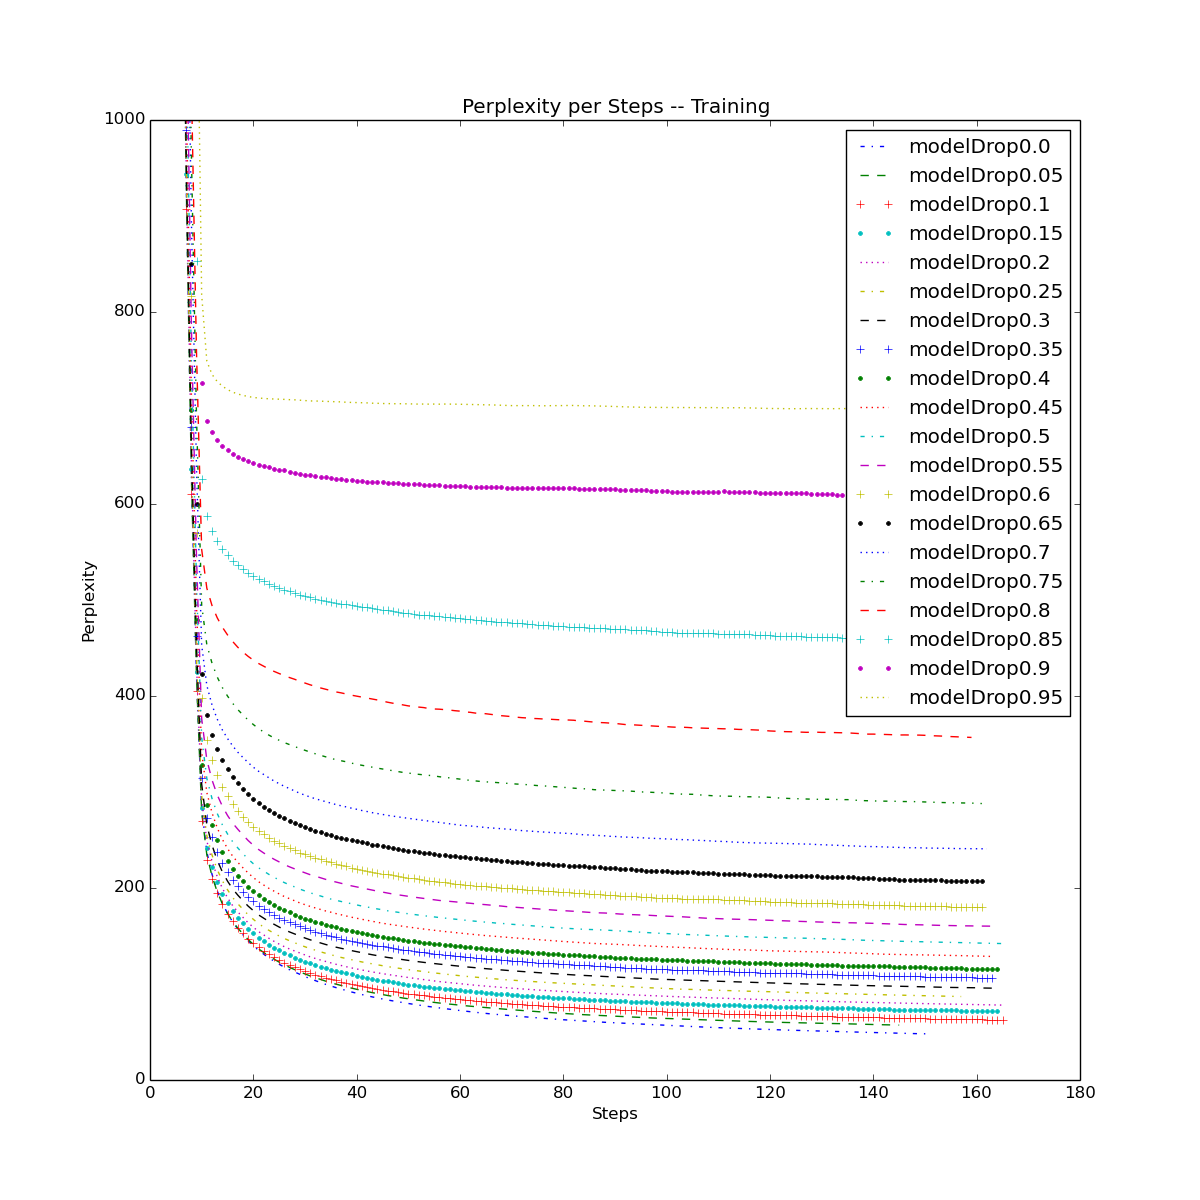
\includegraphics[width = 30mm]{../lstm_me/fig/Drop_train.png}}&
  {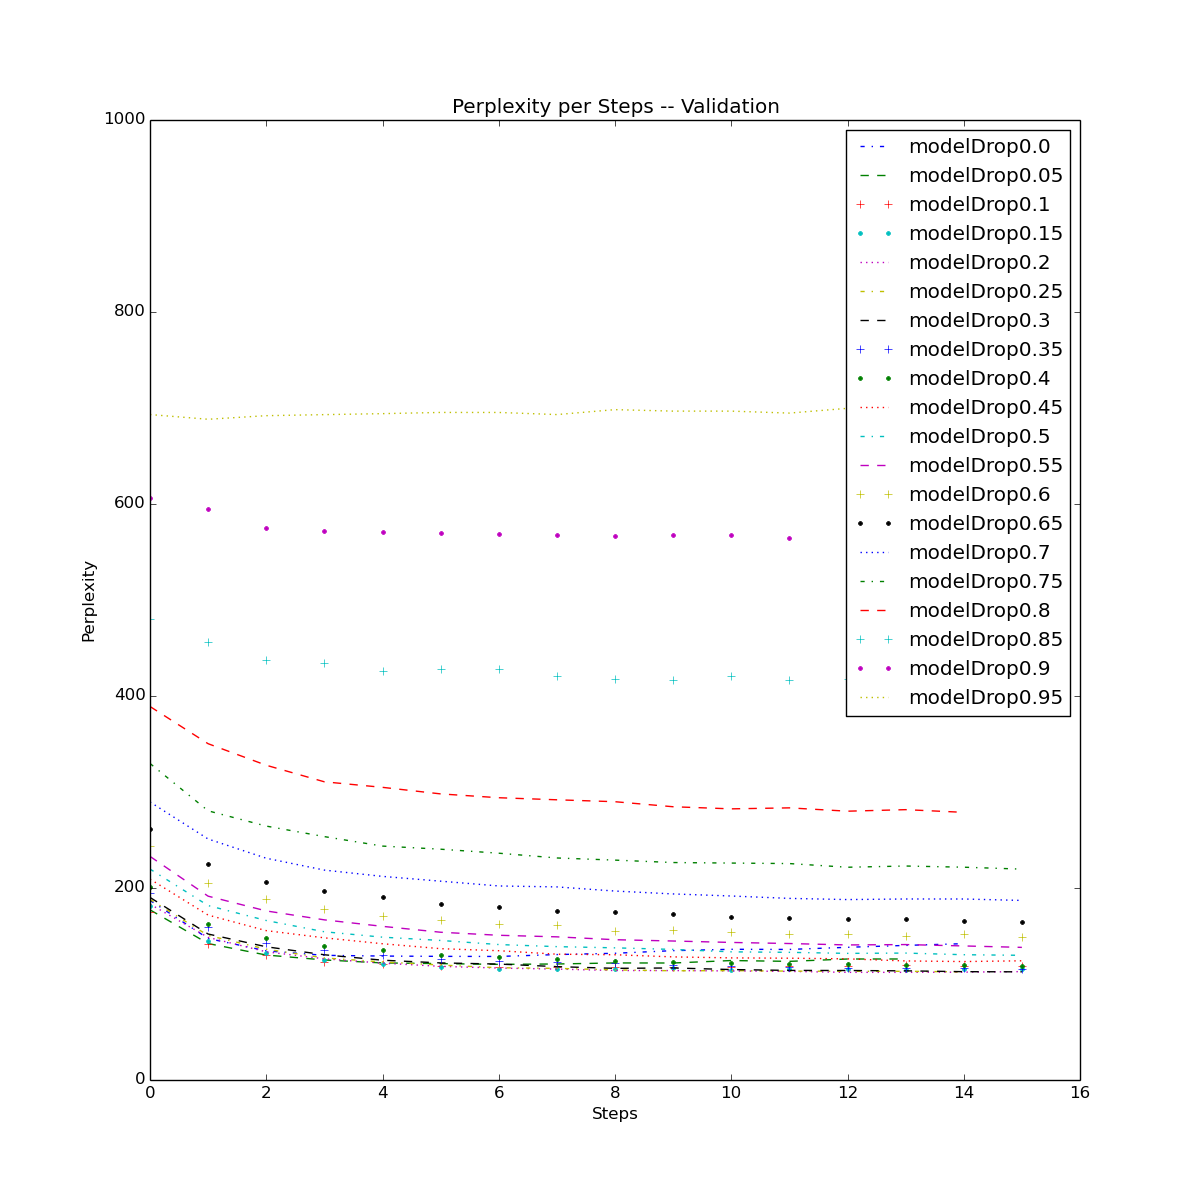
\includegraphics[width = 30mm]{../lstm_me/fig/Drop_val.png}}
  \end{tabular}
\end{subfigure}
\caption{Parameter for dropout rate. Left is for training set. Right is for validation set}
\end{figure}

Second test is about the max gradient norm and its effect on soft or hard clip. There is a trend that the higher the value the later the perplexity goes down. Also the value I tested is higher than default(5), and seems higher value will cause more overfitting. Moreover, I tested the clipping methods on the dropout between 40\% to 50\%, which is the ideal range as mentioned ealier, seems hard clip have no way to further improve the perplexity any further.
\begin{figure}[h]
\centering
\begin{subfigure}
  \begin{tabular}{cccc}
  {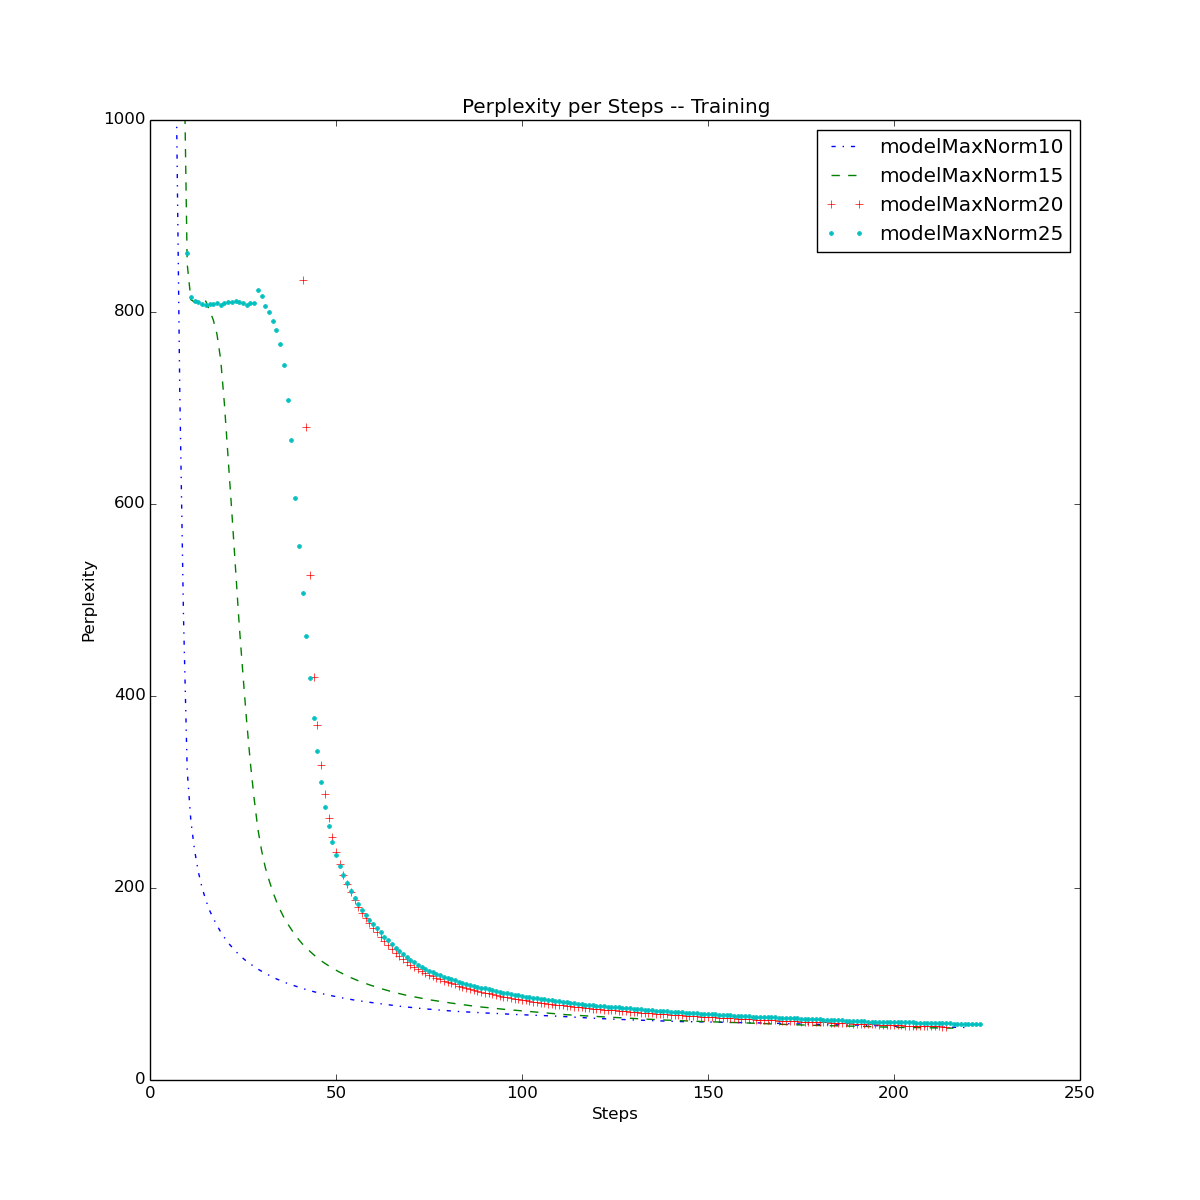
\includegraphics[width = 30mm]{../lstm_me/fig/MaxNorm_train.png}}&
  {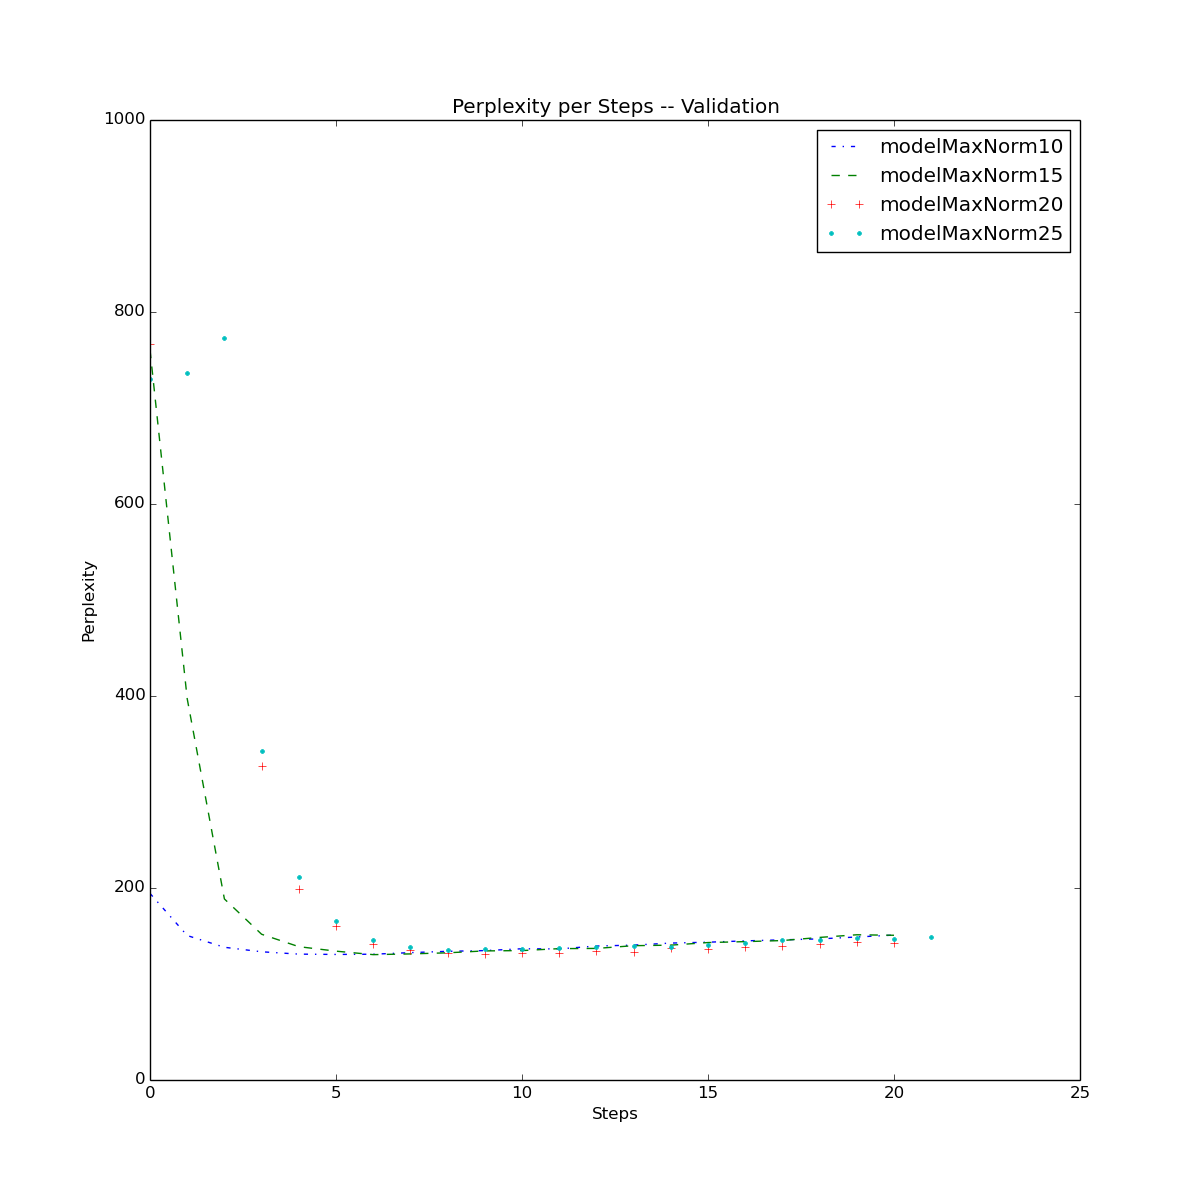
\includegraphics[width = 30mm]{../lstm_me/fig/MaxNorm_val.png}}&
  {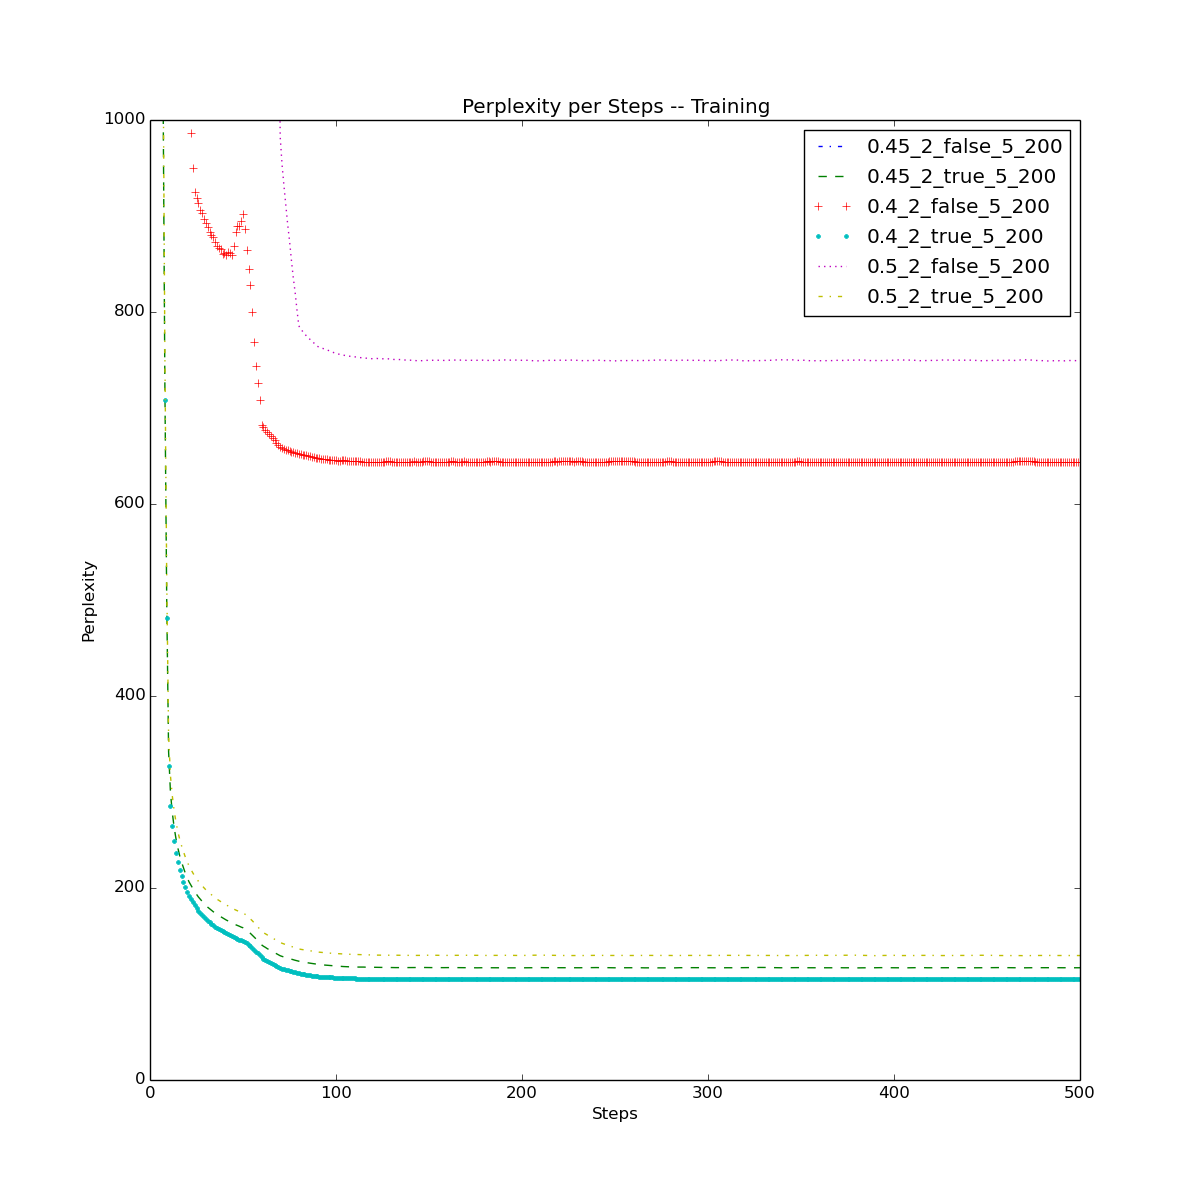
\includegraphics[width = 30mm]{../lstm_me/fig/dropout_clip_train.png}}&
  {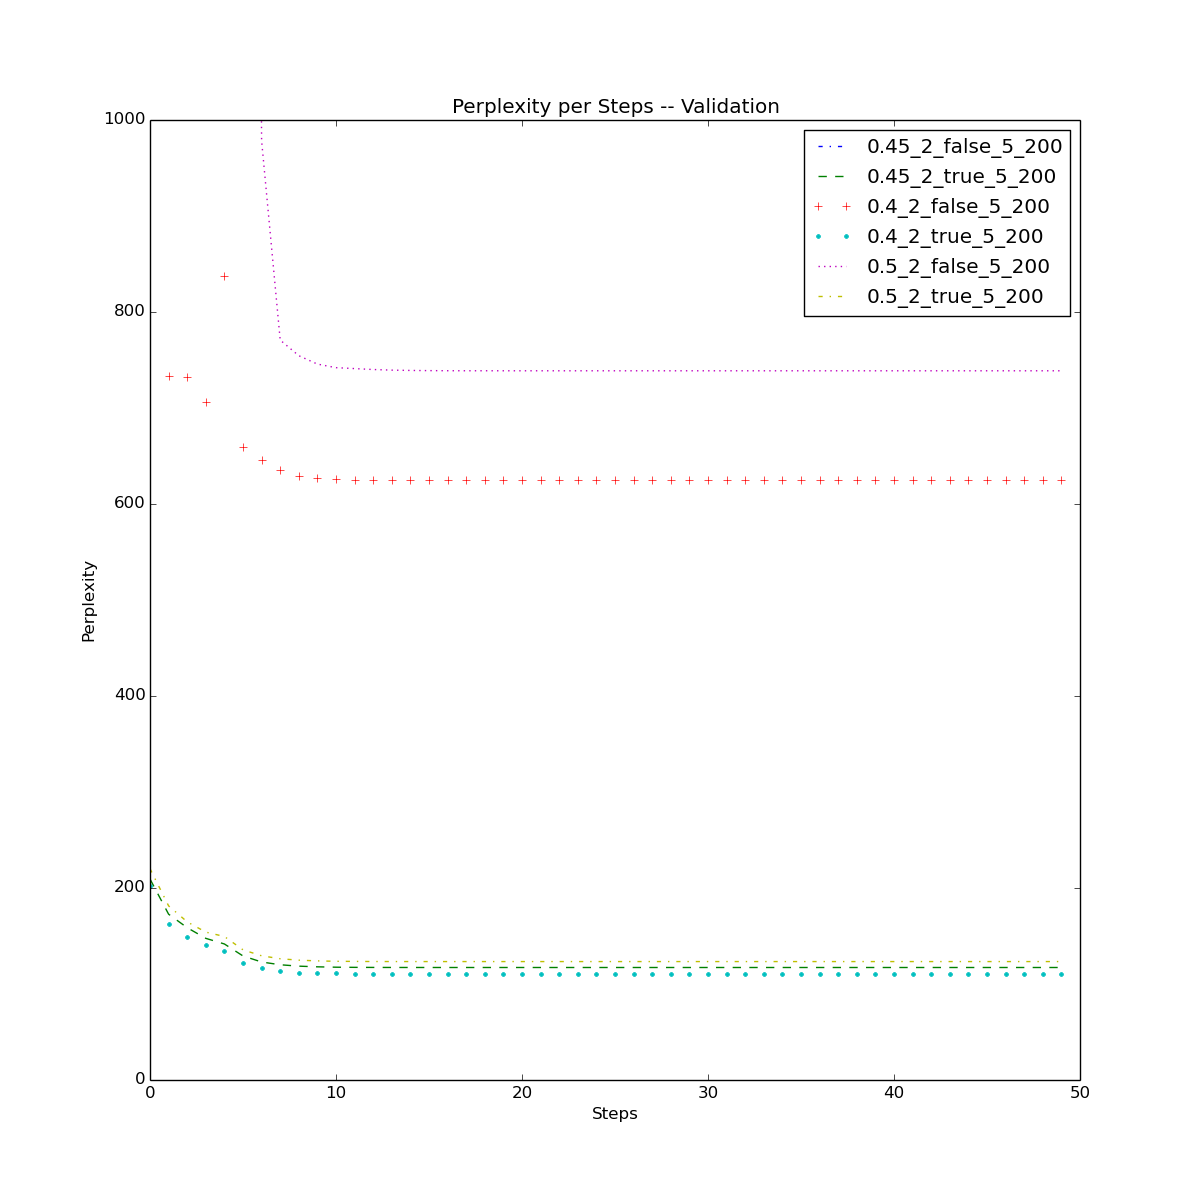
\includegraphics[width = 30mm]{../lstm_me/fig/dropout_clip_val.png}}
  \end{tabular}
\end{subfigure}
\caption{ First and Second are taining and validation with different max gradient norm. Third and fourth are taining and validation with fixed max gradient norm but different dropout and clipping method (true for soft, false for hard clip)}
\end{figure}

Lastly, there are two experiments I like to test, one is number of layers, and the other is number of cnn units. Each layer should compose multiple number of cnn units, and I was wondering what will produce better result if I increase the layer or cnn units. First I did the test for layer ranging from 3 to 10, and actually the result was not as good as 2 layer (data not shown), potentially might due to increasing number of layer also increase much more weightings need to train. Then, instereatingly when testing the combination of 1 or 2 layer with different number of cnn units, I got a better result for using only 1 layer with about 275 cnn units.

\begin{table}[h]
\begin{center}
    \begin{tabular}{| c | c | c | c | c |}
    \hline
    Dropout & Layers & CNN units & Train Perplexity & Test Perplexity\\ \hline
    0.4 & 2 & 275 & 90.252 & 102.006 \\ \hline
    0.4 & 1 & 275 & 79.675 & 97.159 \\ \hline
    0.45 & 2 & 275 & 102.319 & 108.778 \\ \hline
    0.45 & 1 & 275 & 89.991 & 99.737 \\ \hline
    0.5 & 2 & 275 & 113.673 & 113.754 \\ \hline
    0.5 & 1 & 275 & 101.622 & 108.197 \\ \hline
    \end{tabular}
\end{center}
\caption{The training and test accuracy of kmeans implementation based on reference paper}
\end{table}

\begin{figure}[h]
\centering
\begin{subfigure}
  \begin{tabular}{cccc}
  {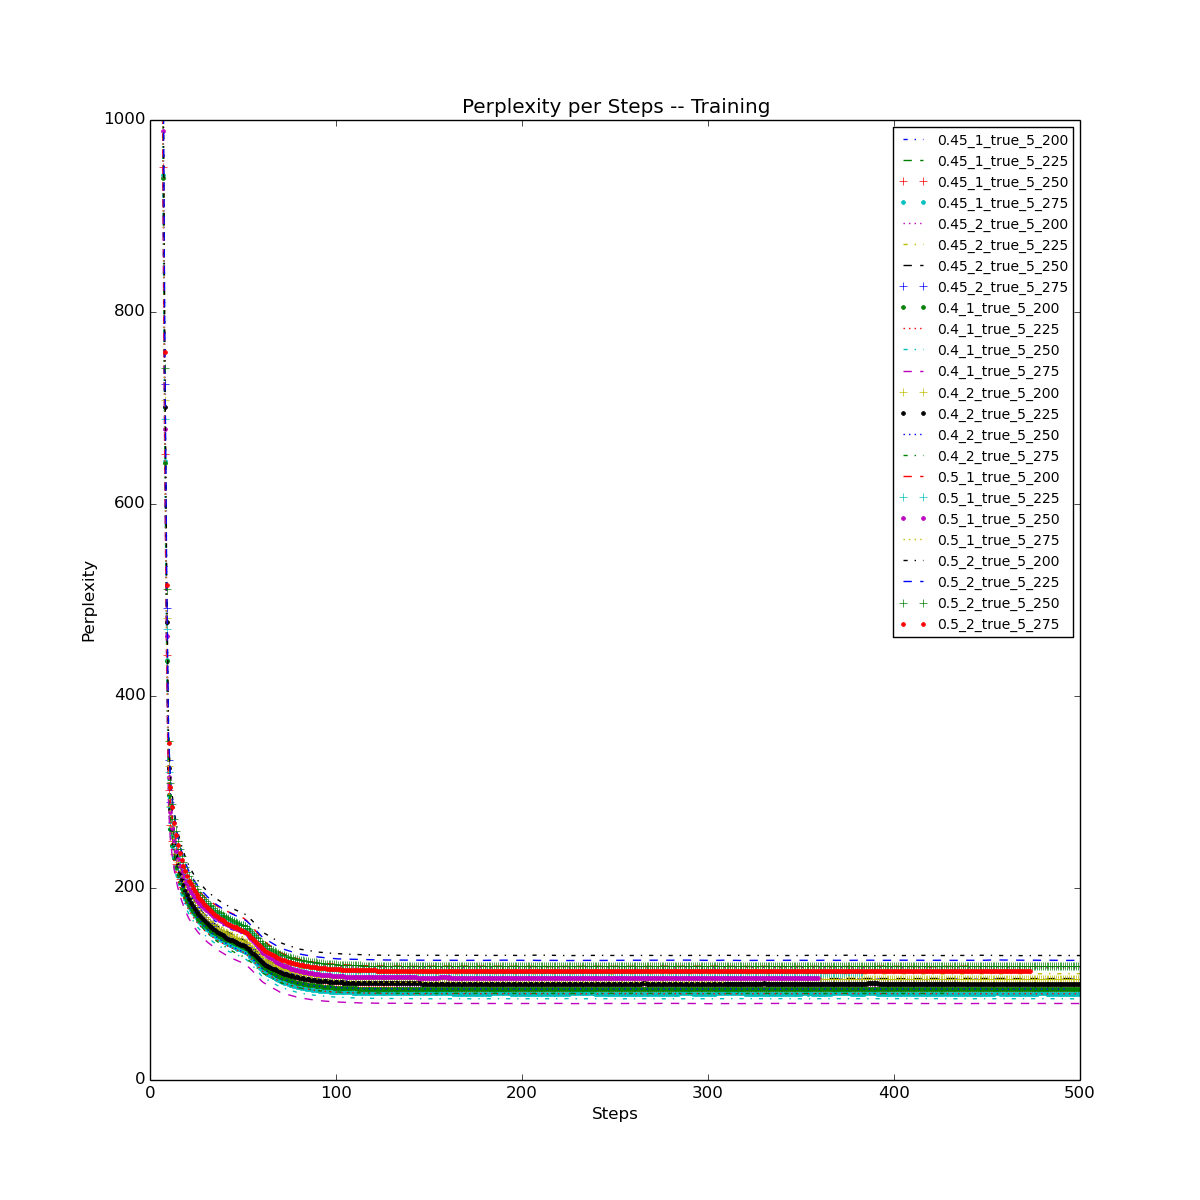
\includegraphics[width = 50mm]{../lstm_me/fig/alltest_onlySoft_train.png}}&
  {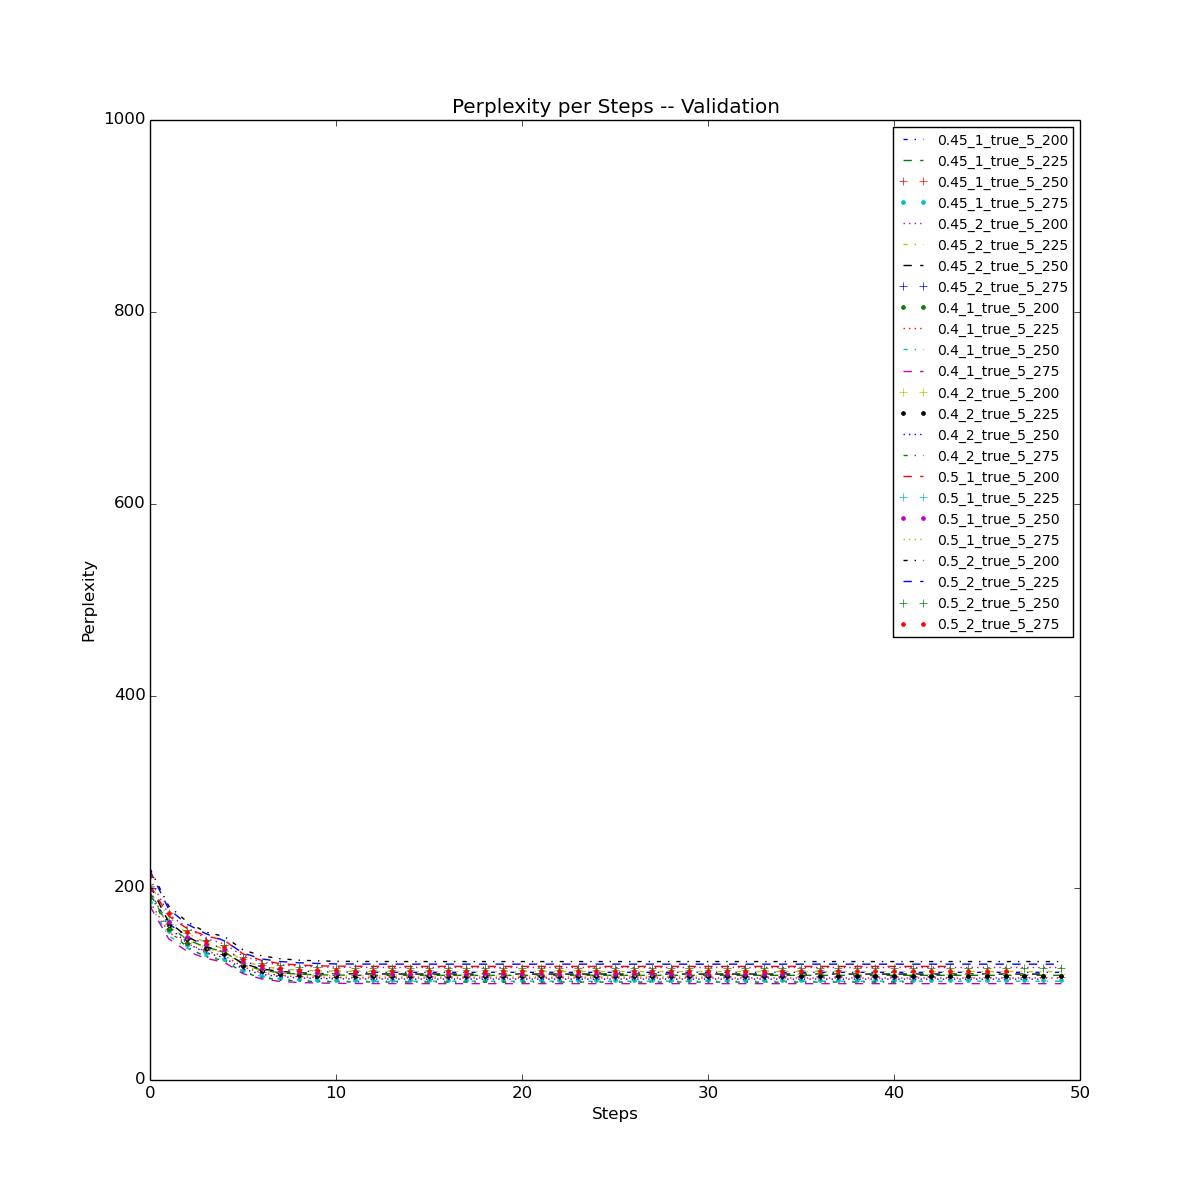
\includegraphics[width = 50mm]{../lstm_me/fig/alltest_onlySoft_val.png}}
  \end{tabular}
\end{subfigure}
\caption{Parameter for dropout, layers, and cnn units. Left is for training set. Right is for validation set}
\end{figure}


\end{document}




